
%(BEGIN_QUESTION)
% Copyright 2010, Tony R. Kuphaldt, released under the Creative Commons Attribution License (v 1.0)
% This means you may do almost anything with this work of mine, so long as you give me proper credit

Examine this motor control circuit, designed to bring the motor to a quick halt whenever the ``Stop'' button is pressed.  The system uses two motor contactors (``F'' and ``R''), each one wired to power the motor in a different direction (forward versus reverse):

$$\includegraphics[width=15.5cm]{i03983x01.eps}$$

Explain how this automatic braking system works.

\vskip 20pt \vbox{\hrule \hbox{\strut \vrule{} {\bf Suggestions for Socratic discussion} \vrule} \hrule}

\begin{itemize}
\item{} Does this braking strategy remind you of one sometimes implemented in VFDs?
\item{} Can you think of any disadvantages to this braking scheme?
\item{} Modify the schematic diagram to contain a hand switch that disables the braking feature.
\item{} Identify any potentially dangerous failure modes in this circuit (i.e. ways in which a component might fail that would make the motor run in a dangerous way).
\item{} Why doesn't the reverse contactor coil (``R'') have OL contacts connected in series like the forward contactor coil (``F'')?
\item{} Identify the consequences of jumpering across the ``R'' contactor coil in this circuit using a piece of wire.
\item{} Identify the consequences of jumpering across the ``F'' contactor coil in this circuit using a piece of wire.
\item{} Identify the consequences of jumpering across the normally-closed ``F'' relay contacts in this circuit using a piece of wire.
\item{} Identify the consequences of jumpering across the normally-open ``F'' relay contacts in this circuit using a piece of wire.
\item{} Identify the consequences of jumpering across the speed switch contacts in this circuit using a piece of wire.
\end{itemize}

\underbar{file i03983}
%(END_QUESTION)





%(BEGIN_ANSWER)


%(END_ANSWER)





%(BEGIN_NOTES)

This motor control circuit uses {\it plugging} to brake the motor.  When the ``Stop'' button is pressed, reverse power is applied to the motor until its forward speed falls below 100 RPM.

\vskip 20pt \vbox{\hrule \hbox{\strut \vrule{} {\bf Virtual Troubleshooting} \vrule} \hrule}

This question is a good candidate for a ``Virtual Troubleshooting'' exercise.  Presenting the diagram to students, you first imagine in your own mind a particular fault in the system.  Then, you present one or more symptoms of that fault (something noticeable by an operator or other user of the system).  Students then propose various diagnostic tests to perform on this system to identify the nature and location of the fault, as though they were technicians trying to troubleshoot the problem.  Your job is to tell them what the result(s) would be for each of the proposed diagnostic tests, documenting those results where all the students can see.

During and after the exercise, it is good to ask students follow-up questions such as:

\begin{itemize}
\item{} What does the result of the last diagnostic test tell you about the fault?
\item{} Suppose the results of the last diagnostic test were different.  What then would that result tell you about the fault?
\item{} Is the last diagnostic test the best one we could do?
\item{} What would be the ideal order of tests, to diagnose the problem in as few steps as possible?
\end{itemize}

%INDEX% Electronics review: AC motor control circuit

%(END_NOTES)

